% Exact copies of revised-manuscript figures and tables used after responses.
% Labels are intentionally omitted so references continue to resolve through
% \externaldocument{main}; captions are unnumbered and show the manuscript ID.

\newcommand{\showMainResults}{%
\begin{table}[!h]
\centering
\small
\caption*{\textbf{Table~\ref{tab:main_results}.} \revised{Main comparison on Intentonomy test split. Avg.\ is the mean of Macro/Micro/Samples F1. FDIL rows report mean$\pm$std over three seeds. $^{\dagger}$Quoted from IntentMLM~\cite{wang_unlocking_2026}.}}
\begingroup
\setlength{\tabcolsep}{4pt}
\begin{tabular}{llcccc}
\hline
Method & Publication & Macro F1 & Micro F1 & Samples F1 & Avg. \\
\hline
Random & - & 6.94 & 7.18 & 7.10 & 7.07 \\
Visual \cite{he_deep_2016} & CVPR 2016 & 22.77 & 30.23 & 28.45 & 27.15 \\
\hline
\multicolumn{6}{l}{\textbf{Multi-label classification methods}} \\
HiMulConE \cite{zhang_use_2022} & CVPR 2022 & 28.43 & 41.50 & 42.15 & 37.36 \\
MultiGuard \cite{jia_multiguard_2022} & NeurIPS 2022 & 26.87 & 38.67 & 40.06 & 35.20 \\
SST \cite{chen_structured_2022} & AAAI 2022 & 27.33 & 42.21 & 42.62 & 37.39 \\
Query2Label \cite{liu_query2label_2021} & - & 32.12 & 44.64 & 45.15 & 40.64 \\
DualCoOp \cite{sun_dualcoop_2022} & NeurIPS 2022 & 31.06 & 44.42 & 40.40 & 38.63 \\
\hline
\multicolumn{6}{l}{\textbf{Label noise methods}} \\
Cleannet \cite{lee_cleannet_2018} & CVPR 2018 & 25.89 & 42.15 & 40.97 & 36.34 \\
LS \cite{lukasik_does_2020} & ICML 2020 & 24.32 & 42.77 & 43.27 & 36.79 \\
Dividemix \cite{li_dividemix_2019} & ICLR 2020 & 30.11 & 40.23 & 41.56 & 37.30 \\
\hline
\multicolumn{6}{l}{\textbf{Intent perception methods}} \\
Jia \cite{jia_intentonomy_2021} & CVPR 2021 & 23.98 & 31.28 & 31.39 & 28.88 \\
CPAD \cite{ye_cross-modality_2023} & TIP 2023 & 27.39 & 40.98 & 41.12 & 36.50 \\
HLEG \cite{shi_learnable_2023} & TAC 2023 & 32.77 & 44.69 & 45.54 & 41.00 \\
\revised{HLEG (CLIP ViT-L/14)} \cite{shi_learnable_2023} & \revised{TAC 2023} & \revised{48.17} & \revised{57.29} & \revised{56.81} & \revised{54.09} \\
PIP-Net \cite{wang_prototype-based_2023} & TMM 2023 & 32.57 & 45.94 & 47.05 & 41.85 \\
LabCR \cite{shi_label-aware_2024} & TIP 2024 & 34.63 & 48.51 & 48.05 & 43.73 \\
\revised{LabCR (CLIP ViT-L/14)} \cite{shi_label-aware_2024} & \revised{TIP 2024} & \revised{48.04} & \revised{57.13} & \revised{56.65} & \revised{53.94} \\
IntCLIP \cite{leonardis_synergy_2025} & ECCV 2024 & 40.15 & 53.54 & 51.01 & 48.23 \\
\revised{IntCLIP (CLIP ViT-L/14)} \cite{leonardis_synergy_2025} & \revised{ECCV 2024} & \revised{47.28} & \revised{56.18} & \revised{54.86} & \revised{52.77} \\
IntentMLM \cite{wang_unlocking_2026} & PR 2026 & 43.05 & 54.77 & 56.75 & 51.52 \\
\hline
\multicolumn{6}{l}{\revised{\textbf{Zero-shot VLM}}} \\
\revised{Qwen3-VL-8B-Instruct \cite{qwen_qwen3-vl_2025}} & \revised{-} & \revised{38.51} & \revised{40.75} & \revised{39.63} & \revised{39.63} \\
\revised{InternVL3-8B \cite{zhu_internvl3_2025}} & \revised{-} & \revised{37.54} & \revised{41.85} & \revised{40.50} & \revised{39.97} \\
\revised{GPT-4o \cite{hurst_gpt-4o_2024}$^{\dagger}$} & \revised{-} & \revised{39.48} & \revised{40.57} & \revised{41.45} & \revised{40.50} \\
\hline
CLIP ViT-L/14 \cite{radford_learning_2021} & ICML 2021 & $47.40$ & $56.42$ & $56.41$ & $53.41$ \\
FDIL (UTD only) & Ours & \revised{$50.20_{\pm0.44}$} & \revised{$58.03_{\pm0.11}$} & \revised{$58.79_{\pm0.78}$} & \revised{$55.68_{\pm0.44}$} \\
FDIL & Ours & \revised{$\mathbf{52.13}_{\pm0.81}$} & \revised{$\mathbf{60.06}_{\pm0.24}$} & \revised{$\mathbf{60.28}_{\pm0.42}$} & \revised{$\mathbf{57.49}_{\pm0.49}$} \\
\hline
\end{tabular}
\endgroup
\end{table}%
}

\newcommand{\showDifficultyResults}{%
\begin{table}[!h]
\centering
\caption*{\textbf{Table~\ref{tab:difficulty_results}.} \revised{Difficulty-based intent subsets (Easy/Medium/Hard); Avg.\ is the subset mean. FDIL is the mean over three seeds.}}
\begin{tabular}{lcccc}
\hline
Method & Easy & Medium & Hard & Avg. \\
\hline
Random & 19.86 & 7.11 & 2.81 & 9.93 \\
Visual \cite{he_deep_2016} & 54.64 & 24.92 & 10.71 & 30.09 \\
Jia (w/o hashtag) \cite{jia_intentonomy_2021} & 57.10 & 25.68 & 12.72 & 31.83 \\
Jia (hashtag) \cite{jia_intentonomy_2021} & 58.86 & 26.30 & 13.11 & 32.76 \\
Query2Label \cite{liu_query2label_2021} & 81.59 & 38.06 & 14.55 & 44.73 \\
CPAD \cite{ye_cross-modality_2023} & 69.47 & 31.50 & 8.54 & 36.50 \\
HLEG \cite{shi_learnable_2023} & 81.49 & 38.99 & 20.22 & 46.90 \\
PIP-Net \cite{wang_prototype-based_2023} & 70.73 & 33.63 & 14.33 & 39.56 \\
IntentMLM \cite{wang_unlocking_2026} & 76.26 & 46.87 & 27.39 & 50.17 \\
\hline
CLIP ViT-L/14 \cite{radford_learning_2021} & 80.99 & 53.32 & 28.45 & 54.25 \\
FDIL & \revised{\textbf{81.19}} & \revised{\textbf{57.73}} & \revised{\textbf{35.02}} & \revised{\textbf{57.98}} \\
\hline
\end{tabular}
\end{table}%
}

\newcommand{\showTsne}{%
\begin{figure}[!h]
\centering
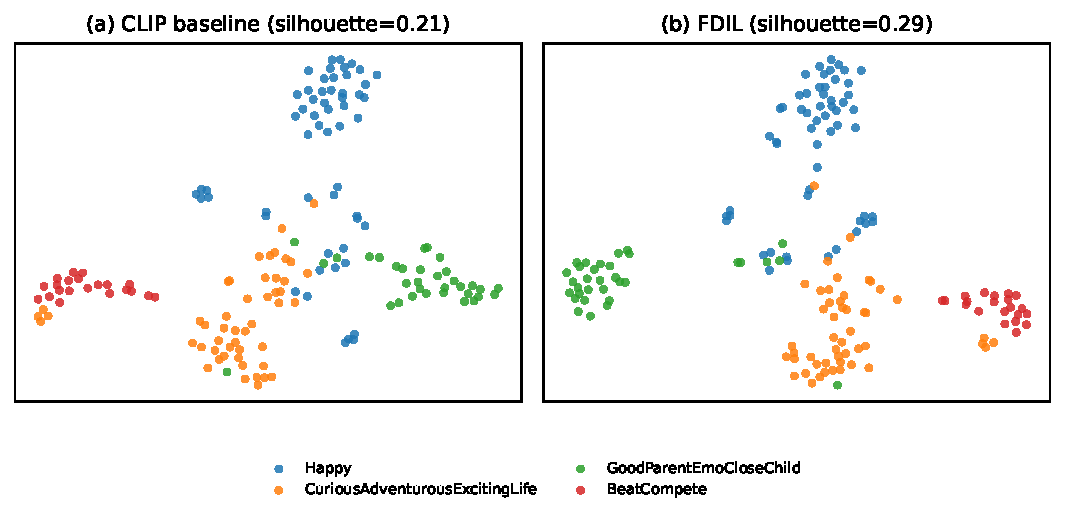
\includegraphics[width=0.9\linewidth]{5_tsne.pdf}
\caption*{\textbf{Figure~\ref{fig:tsne}.} \revised{t-SNE of the decision-score space on four semantically adjacent intents. FDIL yields tighter, better-separated same-intent clusters than the CLIP baseline.}}
\end{figure}%
}

\newcommand{\showPerClassAttr}{%
\begin{table}[!h]
\centering
\small
\caption*{\textbf{Table~\ref{tab:per_class_attr}.} \revised{Per-class F1 attribution of FDIL versus the CLIP baseline (matched class-wise protocol, representative seed). Top: five largest improvements; bottom: the only two regressions among all $28$ classes.}}
\setlength{\tabcolsep}{5pt}
\begin{tabular}{lcccc}
\hline
\revised{Intent class} & \revised{Subset} & \revised{Baseline} & \revised{FDIL} & \revised{$\Delta$} \\
\hline
\revised{WorkILike} & \revised{Hard} & \revised{14.6} & \revised{43.0} & \revised{$+28.5$} \\
\revised{PassionAboutSomething} & \revised{Hard} & \revised{11.3} & \revised{28.6} & \revised{$+17.3$} \\
\revised{SocialLifeFriendship} & \revised{Hard} & \revised{33.9} & \revised{51.2} & \revised{$+17.2$} \\
\revised{ManageableMakePlan} & \revised{Medium} & \revised{17.5} & \revised{32.0} & \revised{$+14.5$} \\
\revised{BeatCompete} & \revised{Medium} & \revised{54.6} & \revised{68.1} & \revised{$+13.5$} \\
\hline
\revised{FineDesignLearnArt-Arch} & \revised{Easy} & \revised{84.0} & \revised{83.1} & \revised{$-1.0$} \\
\revised{CreativeUnique} & \revised{Medium} & \revised{41.9} & \revised{36.6} & \revised{$-5.3$} \\
\hline
\end{tabular}
\end{table}%
}

\newcommand{\showUnifiedDecoupled}{%
\begin{table}[!h]
\centering
\small
\caption*{\textbf{Table~\ref{tab:unified_decoupled}.} \revised{Unified versus functionally decoupled ambiguity handling. Results are means over three seeds.}}
\setlength{\tabcolsep}{4pt}
\begin{tabular}{lccccc}
\hline
\revised{Method} & \revised{Macro} & \revised{Micro} & \revised{Samples} & \revised{Avg.} & \revised{Hard} \\
\hline
\revised{Unified UTD only} & \revised{50.20} & \revised{58.03} & \revised{58.79} & \revised{55.68} & \revised{30.27} \\
\revised{Unified SLR-C only} & \revised{51.29} & \revised{\textbf{60.10}} & \revised{59.22} & \revised{56.87} & \revised{34.01} \\
\revised{Unified joint-target KD} & \revised{50.69} & \revised{58.35} & \revised{57.96} & \revised{55.66} & \revised{32.41} \\
\revised{FDIL (decoupled)} & \revised{\textbf{52.13}} & \revised{60.06} & \revised{\textbf{60.28}} & \revised{\textbf{57.49}} & \revised{\textbf{35.02}} \\
\hline
\end{tabular}
\end{table}%
}

\newcommand{\showPriorAblation}{%
\begin{table}[!h]
\centering
\caption*{\textbf{Table~\ref{tab:prior_ablation}.} \revised{Ablation of textual priors in SLR-C (reranking-only, $K{=}10$). Results use a single seed.}}
\begin{tabular}{cccccccc}
\hline
Lexical & Canonical & Scenario & Macro & Micro & Samples & Avg. & Hard \\
\hline
$\checkmark$ &  &  & \revised{49.76} & \revised{59.12} & \revised{\textbf{58.60}} & \revised{55.83} & \revised{31.22} \\
 & $\checkmark$ &  & \revised{49.80} & \revised{59.50} & \revised{58.05} & \revised{55.78} & \revised{29.88} \\
 &  & $\checkmark$ & \revised{49.35} & \revised{58.88} & \revised{57.87} & \revised{55.37} & \revised{32.48} \\
$\checkmark$ & $\checkmark$ &  & \revised{\textbf{51.18}} & \revised{59.39} & \revised{58.11} & \revised{56.23} & \revised{32.92} \\
$\checkmark$ &  & $\checkmark$ & \revised{50.12} & \revised{59.30} & \revised{58.36} & \revised{55.93} & \revised{32.75} \\
 & $\checkmark$ & $\checkmark$ & \revised{50.93} & \revised{59.51} & \revised{58.18} & \revised{56.21} & \revised{\textbf{34.81}} \\
$\checkmark$ & $\checkmark$ & $\checkmark$ & \revised{50.90} & \revised{\textbf{59.81}} & \revised{58.47} & \revised{\textbf{56.40}} & \revised{32.80} \\
\hline
\end{tabular}
\end{table}%
}

\newcommand{\showKSensitivity}{%
\begin{table}[!h]
\centering
\caption*{\textbf{Table~\ref{tab:k_sensitivity_test}.} \revised{Sensitivity to candidate size $K$ (class-wise thresholding). Results are means over three seeds.}}
\begin{tabular}{lccccc}
\hline
Top-$K$ & Macro & Micro & Samples & Avg. & Hard \\
\hline
5 & \revised{51.19} & \revised{59.03} & \revised{59.42} & \revised{56.54} & \revised{31.60} \\
10 & \revised{\textbf{52.13}} & \revised{\textbf{60.06}} & \revised{\textbf{60.28}} & \revised{\textbf{57.49}} & \revised{\textbf{35.02}} \\
28 & \revised{51.64} & \revised{59.59} & \revised{59.71} & \revised{56.98} & \revised{34.02} \\
\hline
\end{tabular}
\end{table}%
}

\newcommand{\showThresholdingTest}{%
\begin{table}[!h]
\centering
\small
\caption*{\textbf{Table~\ref{tab:thresholding_test}.} \revised{Calibration decomposition under matched global/class-wise thresholding. FDIL is mean$\pm$std over three seeds; CLIP uses a single seed.}}
\setlength{\tabcolsep}{3pt}
\begin{tabular}{llcccccc}
\hline
\revised{Method} & \revised{Threshold} & \revised{Macro} & \revised{Micro} & \revised{Samples} & \revised{Avg.} & \revised{mAP} & \revised{Hard} \\
\hline
\revised{CLIP ViT-L/14 \cite{radford_learning_2021}} & \revised{Global} & \revised{$46.22$} & \revised{$55.05$} & \revised{$54.51$} & \revised{$51.92$} & \revised{$50.67$} & \revised{$26.84$} \\
\revised{CLIP ViT-L/14 \cite{radford_learning_2021}} & \revised{Class-wise} & \revised{$47.40$} & \revised{$56.42$} & \revised{$56.41$} & \revised{$53.41$} & \revised{$50.67$} & \revised{$28.45$} \\
\hline
\revised{FDIL} & \revised{Global} & \revised{$47.70_{\pm1.55}$} & \revised{$57.56_{\pm0.41}$} & \revised{$57.43_{\pm0.69}$} & \revised{$54.23_{\pm0.72}$} & \revised{$\mathbf{55.10}_{\pm0.26}$} & \revised{$30.00_{\pm3.46}$} \\
\revised{FDIL} & \revised{Class-wise} & \revised{$\mathbf{52.13}_{\pm0.81}$} & \revised{$\mathbf{60.06}_{\pm0.24}$} & \revised{$\mathbf{60.28}_{\pm0.42}$} & \revised{$\mathbf{57.49}_{\pm0.49}$} & \revised{$\mathbf{55.10}_{\pm0.26}$} & \revised{$\mathbf{35.02}_{\pm1.77}$} \\
\hline
\end{tabular}
\end{table}%
}

\newcommand{\showThresholdFree}{%
\begin{table}[!h]
\centering
\small
\caption*{\textbf{Table~\ref{tab:threshold_free}.} \revised{Threshold-free, rank-based metrics. mAP is the macro average precision. FDIL/UTD mAP values are means over three seeds; all AUCs and CLIP mAP use a single representative seed.}}
\setlength{\tabcolsep}{4pt}
\begin{tabular}{lcccc}
\hline
\revised{Method} & \revised{mAP} & \revised{Macro ROC-AUC} & \revised{Micro ROC-AUC} & \revised{Micro PR-AUC} \\
\hline
\revised{CLIP ViT-L/14 \cite{radford_learning_2021}} & \revised{50.67} & \revised{87.04} & \revised{84.90} & \revised{54.89} \\
\revised{UTD only} & \revised{53.07} & \revised{\textbf{90.09}} & \revised{\textbf{88.55}} & \revised{59.59} \\
\revised{SLR-C only} & \revised{53.79} & \revised{88.24} & \revised{86.73} & \revised{58.60} \\
\revised{FDIL} & \revised{\textbf{55.10}} & \revised{89.36} & \revised{88.31} & \revised{\textbf{60.64}} \\
\hline
\end{tabular}
\end{table}%
}

\newcommand{\showRocPr}{%
\begin{figure}[!h]
\centering
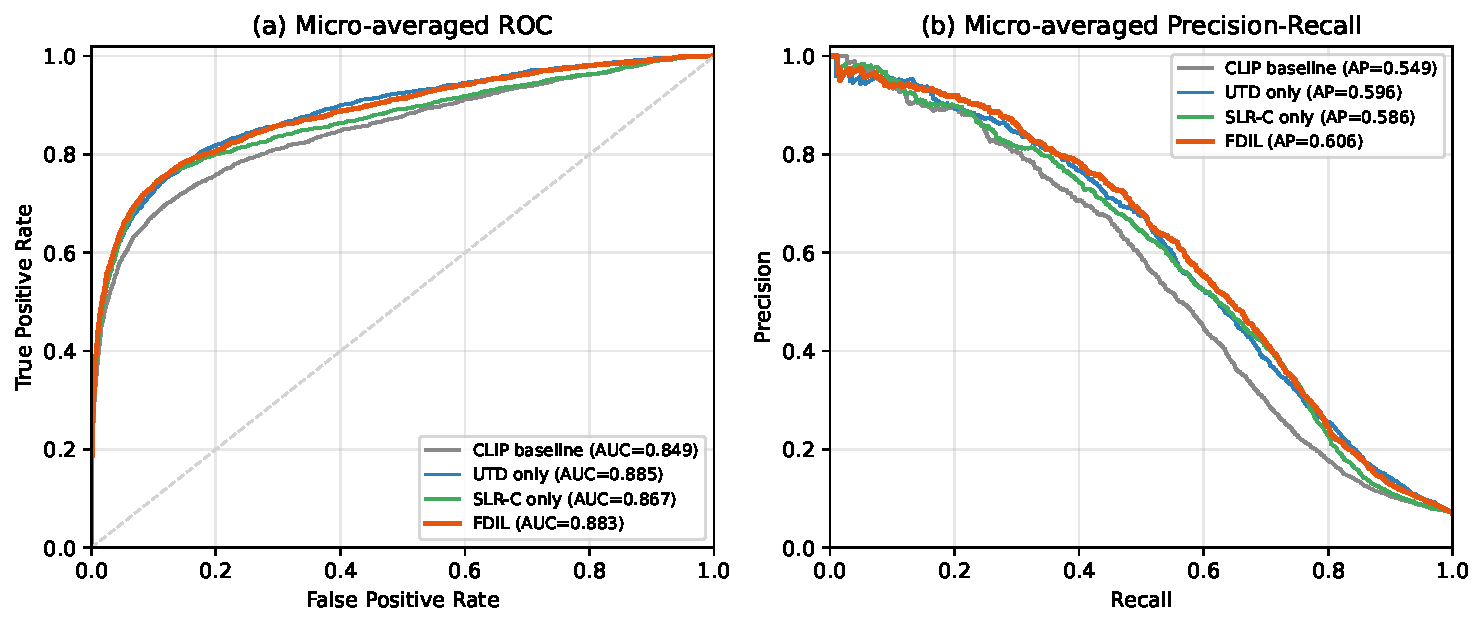
\includegraphics[width=0.9\linewidth]{4_roc_pr.pdf}
\caption*{\textbf{Figure~\ref{fig:roc_pr}.} \revised{Micro-averaged ROC (a) and precision-recall (b) curves, comparing FDIL against the CLIP baseline and three representative methods (HLEG, LabCR, IntCLIP) reproduced under the matched CLIP ViT-L/14 features, split, and protocol.}}
\end{figure}%
}

\newcommand{\showNegativeControls}{%
\begin{table}[!h]
\centering
\small
\caption*{\textbf{Table~\ref{tab:negative_controls}.} \revised{Negative controls on the UTD text teacher ($\Delta$ in points; negative denotes degradation). Full FDIL is the mean over three seeds; control deltas use a single seed.}}
\setlength{\tabcolsep}{4pt}
\begin{tabular}{lcccccc}
\hline
\revised{Condition} & \revised{Macro} & \revised{Micro} & \revised{Samples} & \revised{Avg.} & \revised{mAP} & \revised{Hard} \\
\hline
\revised{FDIL (full)} & \revised{52.13} & \revised{60.06} & \revised{60.28} & \revised{57.49} & \revised{55.10} & \revised{35.02} \\
\revised{\quad w/o UTD (supervised)} & \revised{$-4.03$} & \revised{$-5.59$} & \revised{$-5.17$} & \revised{$-4.94$} & \revised{$-2.18$} & \revised{$-6.02$} \\
\revised{\quad Shuffled rationale} & \revised{$-7.75$} & \revised{$-12.39$} & \revised{$-11.01$} & \revised{$-10.40$} & \revised{$-9.04$} & \revised{$-7.58$} \\
\revised{\quad Ungated teacher} & \revised{$-0.62$} & \revised{$-0.41$} & \revised{$+0.07$} & \revised{$-0.33$} & \revised{$+0.03$} & \revised{$-0.69$} \\
\revised{\quad Uniform agreement gate} & \revised{$-1.16$} & \revised{$-0.93$} & \revised{$-1.21$} & \revised{$-1.12$} & \revised{$-1.33$} & \revised{$+1.13$} \\
\hline
\end{tabular}
\end{table}%
}

\newcommand{\showEfficiencyComparison}{%
\begin{table}[!h]
\centering
\caption*{\textbf{Table~\ref{tab:efficiency_comparison}.} \revised{Feature-level inference cost on frozen CLIP ViT-L/14 features: params (inference-active heads), per-image FLOPs, and batch-1 latency on an RTX 4090.}}
\begin{tabular}{lccc}
\hline
Method & Params (M) & FLOPs (M) & Latency (ms) \\
\hline
Baseline & 1.20 & 2.40 & 0.109 \\
FDIL (UTD only) & 1.20 & 2.40 & 0.109 \\
FDIL & 2.41 & 4.93 & 0.466 \\
\hline
\revised{HLEG \cite{shi_learnable_2023}} & \revised{203.70} & \revised{12\,075.9} & \revised{2.725} \\
\revised{IntCLIP \cite{leonardis_synergy_2025}} & \revised{0.02} & \revised{22.02} & \revised{0.111} \\
\revised{IntentMLM \cite{wang_unlocking_2026}} & \multicolumn{3}{c}{\revised{MLLM: $\sim$10$^{9}$ params, 10--100\,ms/image}} \\
\hline
\end{tabular}
\end{table}%
}

\newcommand{\showFdilFramework}{%
\begin{figure}[!h]
\centering
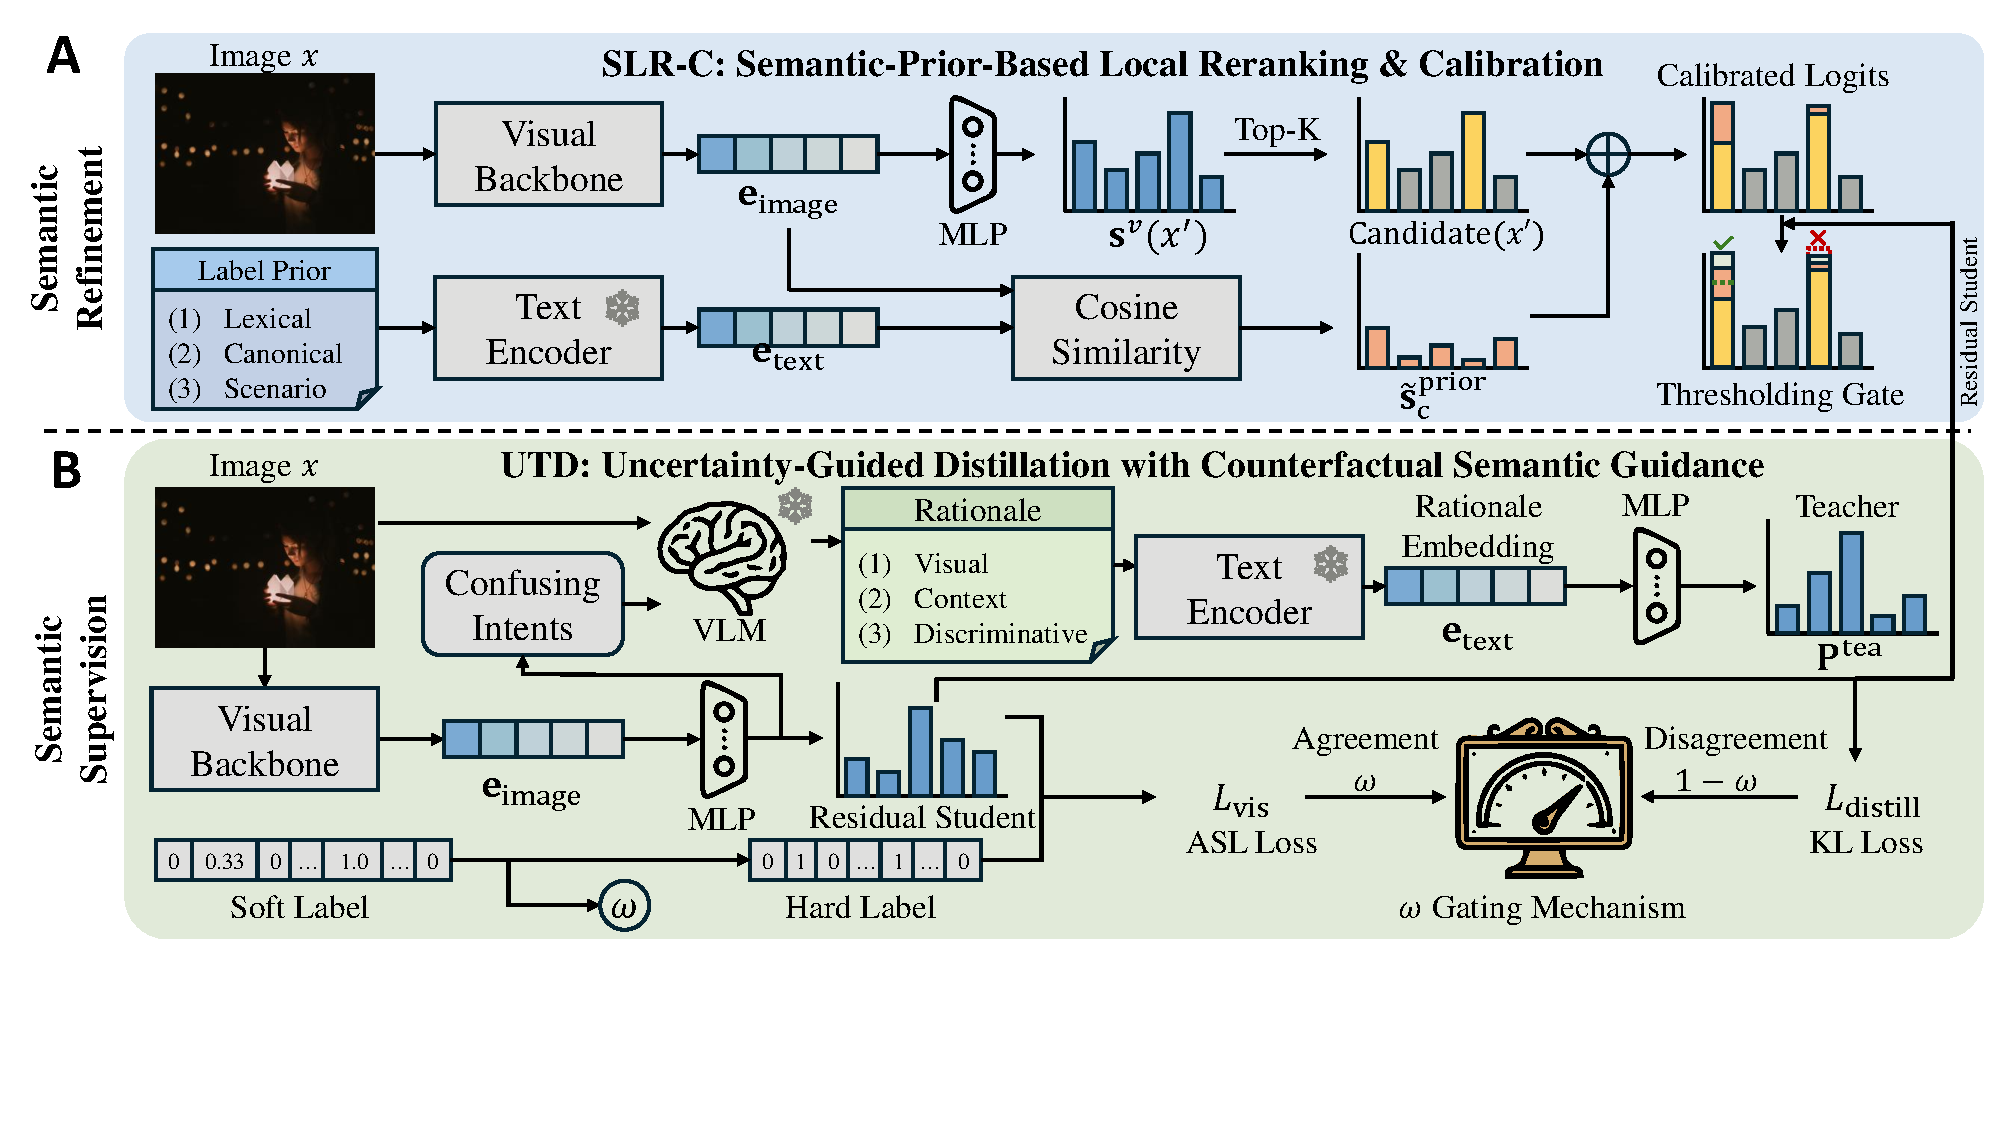
\includegraphics[width=\linewidth]{2_framework.pdf}
\caption*{\textbf{Figure~\ref{fig:fdil_framework}.} \revised{Overview of FDIL. SLR-C constructs a textual semantic prior and performs local reranking plus residual refinement. UTD uses a rationale-based text teacher and an agreement-aware gate to stabilize learning under ambiguous supervision.}}
\end{figure}%
}

\newcommand{\showNotation}{%
\begin{table}[!h]
\centering
\small
\caption*{\textbf{Table~\ref{tab:notation}.} \revised{Key notation used in the method.}}
\setlength{\tabcolsep}{6pt}
\revised{
\begin{tabular}{ll}
\hline
Symbol & Meaning \\
\hline
$x$ & input image \\
$\mathcal{Y},\,C$ & intent label space and number of classes \\
$\mathbf{y}^{\text{soft}},\,\mathbf{y}^{\text{hard}}$ & soft annotation / binarized hard labels \\
$\omega\in(0,1]$ & sample-level annotator agreement score \\
$\phi=f_{\text{img}}(x)$ & frozen visual image feature \\
$\tilde{s}^{\text{prior}}_c$ & normalized heterogeneous semantic prior \\
$\mathcal{C}_K(x),\,K$ & Top-$K$ candidate set and its size \\
$s^{\text{full}}_c$ & final refined score for class $c$ \\
$t_c$ & class-wise decision threshold (validation-only) \\
$\mathbf{p}^{\text{tea}},\,\tau$ & text-teacher distribution and temperature \\
$g=1-\omega$ & teacher-branch gate weight \\
$\mathcal{L}_{\text{total}}$ & total training loss \\
\hline
\end{tabular}
}
\end{table}%
}
